\chapter{From Last Scattering to Baryogenesis}

We begin where Leonard Susskind begins: not with a speculative microphysical mechanism, but with the sky at different distances. Farther out means earlier, and earlier means denser and hotter. From that observational starting point the lecture moves through last scattering, then farther back into pair production and the quark--antiquark soup, then stops, turns the movie around, and asks why any matter was left over at all. These notes follow that order closely and retain selected board evidence from the lecture record prepared with LazyingArt LLC and Video2Book.

\section{Looking Outward Means Looking Backward}

The lecture opens with a very simple geometric idea. We put ourselves at the center, draw shells at larger and larger distances, and ask what we see. Nearby, the look-back time is negligible. The universe a year ago, or a hundred years ago, is not very different from the universe now. But once we look far enough, distance becomes time depth: the farther we look, the younger the universe we are seeing.

And once the universe is younger, it is denser; once it is denser, it is hotter. Susskind fixes the discussion with an order-of-magnitude landmark: if we look back far enough, we reach a place where the universe was about as hot as the surface of the sun. The sky does not \emph{look} like the surface of the sun because the photons have been redshifted on their way to us. At the level needed in this lecture, we may summarize the relation by
\begin{equation}
T_{\mathrm{obs}} \sim \frac{T_{\mathrm{emit}}}{1+z},
\end{equation}
and for the last-scattering epoch the lecture uses the rough scale
\begin{equation}
1+z \sim 10^3.
\end{equation}
So the temperature we observe in the sky is lower by about three orders of magnitude than the temperature at emission.

This is already the right cosmological attitude. We are not simply \emph{told} that the early universe was hot. We are pushed toward that conclusion by the ordinary act of looking outward.

\section{Last Scattering, Ionization, and Opacity}

The first real threshold in the lecture is not baryogenesis but visibility. Hydrogen remains ionized above a temperature of order a few thousand kelvin. Thus when we look back beyond a certain distance, we do not find neutral atoms. We find an ionized gas of nuclei and free electrons, immersed in a sea of energetic photons.

\begin{definition}
The \emph{surface of last scattering} is the transition surface at which the universe changes from an opaque ionized plasma to a transparent gas of neutral atoms.
\end{definition}

The lecture's physical picture is vivid. The universe at that stage is mainly hydrogen, with a little helium. Above the ionization temperature, hydrogen does not remain bound into atoms. We have protons and electrons moving freely. In addition, the photons are shorter-wavelength and more energetic than they are today. If by accident an atom forms, it is quickly struck and reionized again.

That is why the medium is opaque. Ionized gas is an electrical conductor. Free charges respond to electric fields, slosh back and forth, and re-emit radiation. In that state the universe is not transparent. The transition is therefore
\begin{align}
T \gtrsim \text{a few}\times 10^3\ \mathrm{K}
&\quad \Longrightarrow \quad
\text{ionized plasma, opaque},
\\[4pt]
T \lesssim \text{a few}\times 10^3\ \mathrm{K}
&\quad \Longrightarrow \quad
\text{neutral atoms, transparent}.
\end{align}

Susskind compares this to the visible surface of the sun: not a hard material wall, but a place where one suddenly goes from opaque to transparent. Once the temperature drops below the hydrogen ionization scale, the universe clears and we can see through it.

That is the first observational boundary. Behind it, direct vision gives out. But the lecture does not stop there. Having explained why we cannot see farther, it immediately asks: how far can we nevertheless go by using known laws of atomic, nuclear, and particle physics?

\section{Going Further Back: Pair Production and Thermal Thresholds}

At the surface of last scattering the contents are still comparatively simple: mostly photons, with protons and electrons providing the charged matter content, and practically no positrons or antiprotons. But as we continue backward in time, the photons become more and more energetic. Eventually two photons can collide and produce an electron--positron pair:
\begin{equation}
\gamma + \gamma \leftrightarrow e^- + e^+.
\end{equation}
The board records the threshold in its simplest lecture-level form:
\begin{equation}
E_{\gamma\gamma} \ge 2m_e c^2.
\end{equation}

What matters here is not a fully invariant kinematic derivation, but the threshold logic. Below threshold, the photons do not have enough energy. Just above threshold, pairs can be made, but photons still dominate by number because electron rest mass is expensive. Far above threshold, however, that rest mass becomes less and less important relative to thermal kinetic energy, and the densities become comparable:
\begin{equation}
n_\gamma \sim n_{e^-} \sim n_{e^+}.
\end{equation}

\begin{figure}[ht]
\centering

\includegraphics[width=0.62\textwidth]{lecture_06_figure_02.png}
\caption{Electron--positron threshold sketch on the board. The upper threshold annotation \(2m_e c^2\) is clear. The lower proton-scale note is less sharp in the frame, but the transcript makes the intended comparison unmistakable.}
\end{figure}

\begin{figure}[ht]
\centering
\begin{tikzpicture}[scale=1.0]
\draw[->] (-3,1.2) -- (-0.8,0.35);
\draw[->] (-3,-1.2) -- (-0.8,-0.35);
\filldraw (0,0) circle (1.2pt);
\draw (-0.8,0.35) -- (0,0) -- (0.8,0.35);
\draw (-0.8,-0.35) -- (0,0) -- (0.8,-0.35);
\draw[->] (0.8,0.35) -- (3,1.2);
\draw[->] (0.8,-0.35) -- (3,-1.2);

\node at (-2.25,1.55) {$\gamma$};
\node at (-2.25,-1.55) {$\gamma$};
\node at (2.25,1.55) {$e^-$};
\node at (2.25,-1.55) {$e^+$};

\node at (5.5,0.8) {$E_{\gamma\gamma}\ge 2m_e c^2$};
\node at (5.5,-0.8) {$E_{\gamma\gamma}\gtrsim 2m_p c^2$};

\node at (1.8,-2.1) {$\gamma+\gamma \leftrightarrow e^-+e^+$};
\end{tikzpicture}
\caption{Clean reconstruction of the threshold comparison discussed in the lecture. The board image supplies the documentary evidence; the TikZ sketch only cleans up the process and the two mass scales.}
\end{figure}

The lecture then asks the next natural question: what about protons? The answer is that the proton scale lies far higher,
\begin{equation}
E_{\gamma\gamma} \gtrsim 2m_p c^2,
\qquad
m_p \approx 2000\,m_e.
\end{equation}
So there is a long interval in temperature where electrons and positrons are already copious while proton--antiproton pair creation is still negligible.

But even this proton language is only provisional. By the time the temperature is high enough to make proton--antiproton pairs in abundance, it is already high enough to shatter protons. That is why the lecture switches, at the hotter stage, from protons to quarks and antiquarks. The simplest schematic reaction he draws is
\begin{equation}
e^- + e^+ \to \gamma \to q + \bar q.
\end{equation}
There are also gluons, neutrinos, and many other species, but the main point is the thermal logic: once we are far enough back, the soup contains nearly equal abundances of particles and antiparticles of each type, and in order-of-magnitude terms
\begin{equation}
n_q \sim n_{\bar q} \sim n_\gamma.
\end{equation}

For the moment, however, the lecture does not want to drown in particle nomenclature. When it comes time to discuss the asymmetry, it deliberately simplifies back to protons and antiprotons as a stand-in for baryons and antibaryons.

\section{Charge Neutrality and the Symmetric Hot Soup}

Before the asymmetry problem can even be stated correctly, the lecture pauses over a distinction that is easy to miss.

The first statement is electrical neutrality. Today the universe appears electrically neutral. That means the total positive and total negative charge cancel. It does \emph{not} mean that protons and antiprotons are equally numerous.

Susskind's mnemonic for this is the flux picture on a closed spherical universe. If electric field lines cannot simply end in empty space, then a positive charge cannot sit by itself on a closed space without the flux refocusing somewhere and terminating on negative charge. Whether or not our universe is literally a closed three-sphere is not the point. The point is that net charge is extraordinarily constrained. In symbols,
\begin{equation}
Q_{\mathrm{tot}}=0.
\end{equation}

But \(Q_{\mathrm{tot}}=0\) is not the same statement as \(N_p=N_{\bar p}\). Electrical neutrality means that protons, positrons, and all other positively charged species together balance electrons and all other negatively charged species together.

The baryon bookkeeping is different.

\begin{definition}
The baryon number is the net count of baryons minus antibaryons. For the simplified discussion in this lecture we may write
\begin{equation}
B = N_b - N_{\bar b},
\end{equation}
or more explicitly,
\begin{equation}
B=(N_p+N_n)-(N_{\bar p}+N_{\bar n}).
\end{equation}
\end{definition}

At sufficiently high temperature the pair-production processes drive us toward a hot soup in which particles and antiparticles are nearly equally abundant. Susskind is careful here. This is not a theorem about the beginning of the universe. It is the natural starting hypothesis suggested by the near symmetry of known particle physics and by the way thermal pair production works. Electrons and positrons are made together; quarks and antiquarks are made together. Thus, after simplifying back from quarks to protons for the sake of the story, the lecture asks us to imagine an early state with
\begin{equation}
N_p = N_{\bar p}.
\end{equation}

This is now the real setup. We have a nearly symmetric hot soup, electrically neutral, and almost symmetric under exchange of particles and antiparticles. ``Almost'' is the right word. The laws of physics are not exactly symmetric in that way, but they are close enough that the lecture can sharpen the problem without caricaturing it.

Up to this point we have been walking backward in time. The lecturer then stops and says, in effect: the real sequence is the other way around. Now let us run the movie forward.

\section{Turning the Movie Around: Cooling, Annihilation, and Freeze-Out}

The forward story is the cooling story. While the universe is hot enough, pair creation and annihilation both occur. Once the temperature drops below the relevant threshold, the inverse reaction shuts off first, while annihilation can continue. This is what the lecture calls the ``one-way street.''

Consider first the proton channel. While the temperature is sufficiently high, we have
\begin{equation}
p+\bar p \leftrightarrow \gamma+\gamma.
\end{equation}
As the universe expands, the photons are redshifted. Very soon they no longer have enough energy to climb back over the proton threshold, and what remains effectively is
\begin{equation}
p+\bar p \to \gamma+\gamma.
\end{equation}
Exactly the same logic later applies to electrons and positrons:
\begin{equation}
e^-+e^+ \to \gamma+\gamma.
\end{equation}

\begin{figure}[ht]
\centering
\resizebox{\linewidth}{!}{%
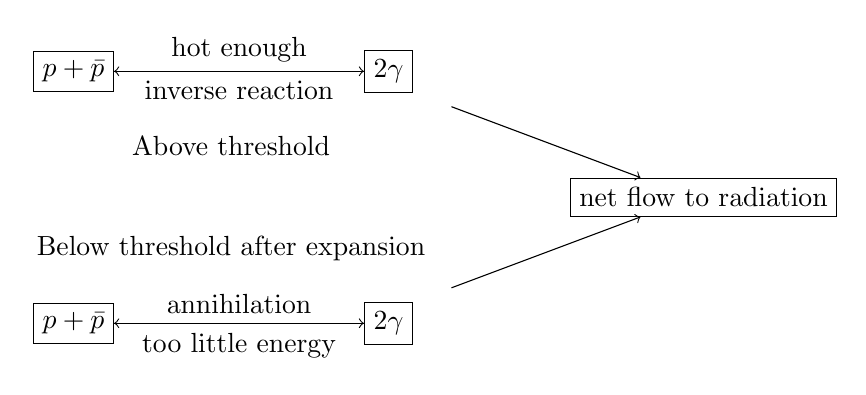
\begin{tikzpicture}[scale=1.0]
\node[draw,rectangle] (a1) at (-4,1.6) {$p+\bar p$};
\node[draw,rectangle] (b1) at (0,1.6) {$2\gamma$};
\draw[->] (a1) -- node[above] {hot enough} (b1);
\draw[->] (b1) -- node[below] {inverse reaction} (a1);

\node at (-2,0.65) {Above threshold};

\node[draw,rectangle] (a2) at (-4,-1.6) {$p+\bar p$};
\node[draw,rectangle] (b2) at (0,-1.6) {$2\gamma$};
\draw[->] (a2) -- node[above] {annihilation} (b2);
\draw[->,dashed] (b2) -- node[below] {too little energy} (a2);

\node at (-2,-0.65) {Below threshold after expansion};

\node[draw,rectangle] (c) at (4,0) {net flow to radiation};
\draw[->] (0.8,1.15) -- (3.2,0.25);
\draw[->] (0.8,-1.15) -- (3.2,-0.25);
\end{tikzpicture}
}%
\caption{The ``one-way street'' of freeze-out. Above threshold the reaction runs both ways. After expansion lowers photon energies, annihilation still proceeds but inverse production is thermally suppressed.}
\end{figure}

There is a small but very useful piece of arithmetic here. A proton--antiproton annihilation event changes the counts by
\begin{align}
N_p &\to N_p-1,\\
N_{\bar p} &\to N_{\bar p}-1,\\
N_\gamma &\to N_\gamma+2.
\end{align}
Therefore the difference stays fixed:
\begin{equation}
(N_p-N_{\bar p}) \to (N_p-1)-(N_{\bar p}-1)=N_p-N_{\bar p}.
\end{equation}
This is the mathematical heart of the freeze-out story. Ordinary annihilation does not \emph{create} a proton excess. It merely strips away matched pairs and leaves any pre-existing difference exposed.

A concrete example makes the point completely transparent. Suppose at some early time
\begin{equation}
N_p^{\mathrm{initial}}=N+\Delta,
\qquad
N_{\bar p}^{\mathrm{initial}}=N,
\end{equation}
with \(\Delta>0\). After all possible annihilations have occurred, one finds
\begin{equation}
N_p^{\mathrm{final}}=\Delta,
\qquad
N_{\bar p}^{\mathrm{final}}=0.
\end{equation}
What survives is precisely the initial excess.

The lecture then folds thermodynamics into the picture. The expansion is slow compared with microscopic reaction rates, so to a good approximation it is adiabatic:
\begin{equation}
S \approx \text{const.}
\end{equation}
Strictly speaking it is the entropy that is conserved, not the particle count itself. But for a thermal gas of the sort being discussed, and especially for blackbody radiation, the entropy is, up to order-one factors, essentially the number of particles, in practice the number of photons. Thus the particles that disappear in annihilation are largely replaced by photons.

That is why the present photon bath is a fossil record of the earlier annihilation history. The lecture uses the present-day count
\begin{equation}
\frac{N_\gamma}{N_p}\sim 10^9\text{--}10^{10}.
\end{equation}
Since today \(N_{\bar p}\) is negligible, we may also phrase the same information as
\begin{equation}
\frac{N_p-N_{\bar p}}{N_\gamma}\sim 10^{-9}\text{--}10^{-10}.
\end{equation}
So the asymmetry was not of order one. It was tiny: about one extra proton for every billion proton--antiproton pairs.

That numerical fact changes the entire tone of the discussion. We are no longer asking why a matter universe did not annihilate away. We are asking how such an absurdly small but nonzero difference could ever have been produced.

\section{Baryogenesis and the Sakharov Conditions}

The lecture now raises the central obstacle very explicitly: if we begin with a nearly symmetric hot soup, why is there any residue at all?

\subsection{Question \& Answer}

\paragraph{Question.} Suppose we start from a perfectly symmetric state,
\begin{equation}
N_p=N_{\bar p},
\end{equation}
and let the universe cool. Why can ordinary physics not generate a tiny extra proton population during cooling? And if not that, could the observed excess simply be a statistical fluctuation?

\paragraph{Answer.} Ordinary cooling cannot do the job. We have already seen that pair annihilation preserves \(N_p-N_{\bar p}\). So if we start from zero difference, annihilation alone leaves us with zero difference. To get one extra proton we would need a process that changes the net baryon number.

Electric charge is not the obstruction. One could imagine, schematically, a process of the form
\begin{equation}
\gamma+\gamma \to p+e^-,
\end{equation}
which is electrically neutral overall. But that is precisely the kind of process that the tested standard model does \emph{not} contain. Within the regime where laboratory particle physics is known to work, one cannot create a proton without also creating an antiproton. That empirical rule is baryon-number conservation.

In the lecture's simplified bookkeeping,
\begin{equation}
B=(N_p+N_n)-(N_{\bar p}+N_{\bar n}),
\end{equation}
and within tested particle physics \(B\) is conserved. So once the temperature has fallen into the range where we trust the standard model, there is no ordinary low-energy route by which a proton excess can develop during cooling.

What about statistics? Could a random freeze-out leave a net excess just by fluctuation? The lecture answers this in the standard square-root-of-\(N\) way:
\begin{equation}
\Delta N_{\mathrm{stat}}\sim \sqrt{N}.
\end{equation}
If we count all particles in the observable universe, including photons, the lecture uses the rough scale \(N\sim 10^{90}\), so
\begin{equation}
\sqrt{10^{90}}\sim 10^{45}.
\end{equation}
But the actual proton count is of order \(10^{80}\). Thus the fluctuation estimate is hopelessly too small:
\begin{equation}
10^{45}\ll 10^{80}.
\end{equation}
So the present matter excess is not a statistical accident of an otherwise unbiased world.

\begin{figure}[ht]
\centering

\includegraphics[width=0.72\textwidth]{lecture_06_figure_03.png}
\caption{Board state during the transition from the residual asymmetry \(N_p-N_{\bar p}\) to the developing numbered list of conditions. The screenshot is useful mainly as documentary evidence for the board's organization.}
\end{figure}

Once those escape routes are closed, the lecture turns constructive. If the asymmetry is real, what must the laws of nature have allowed at very high temperature?

The board now acquires its characteristic shape. First the symmetric starting point,
\begin{equation}
N_p=N_{\bar p},
\end{equation}
then the leftover difference,
\begin{equation}
N_p-N_{\bar p},
\end{equation}
and then the numbered list of conditions under which one can get from the first expression to the second.

\begin{figure}[ht]
\centering

\includegraphics[width=0.72\textwidth]{lecture_06_figure_04.png}
\caption{Asymmetry conditions and checklist on the board. The numbered items are reconstructed from the transcript rather than read directly from the incomplete pixels.}
\end{figure}

The first condition is baryon-number violation. If \(B\) is exactly conserved, then a baryon-neutral universe stays baryon-neutral forever.

The second condition is a bias between particles and antiparticles. The lecture first phrases this loosely as violation of charge-conjugation symmetry and later, correctly, sharpens it to CP violation. The reason is simple. Even if baryon number is violated, it could be violated symmetrically. Schematically, one might have
\begin{align}
\gamma+\gamma &\to p+e^-,
\\
\gamma+\gamma &\to \bar p+e^+.
\end{align}
If those two channels occur with equal average probability, the net asymmetry still vanishes. Baryon violation by itself is therefore not enough; one also needs a bias.

The third condition is departure from thermal equilibrium. Here the lecture invokes the CPT theorem in its conceptual form. In thermal equilibrium a movie run backward looks like the same movie run forward. If, in addition, the underlying theory is exactly symmetric under the combined CPT operation, then equilibrium effectively restores the particle--antiparticle symmetry that we are trying to break. A hot static pot cannot maintain a persistent proton excess. Therefore baryogenesis requires an epoch in which the universe is sufficiently out of equilibrium that forward and backward histories are microscopically distinguishable.

This is the Sakharov structure:
\begin{enumerate}
\item \textbf{Violation of baryon number;}
\item \textbf{Violation of particle--antiparticle symmetry, more precisely CP violation;}
\item \textbf{Departure from thermal equilibrium.}
\end{enumerate}

\begin{figure}[ht]
\centering
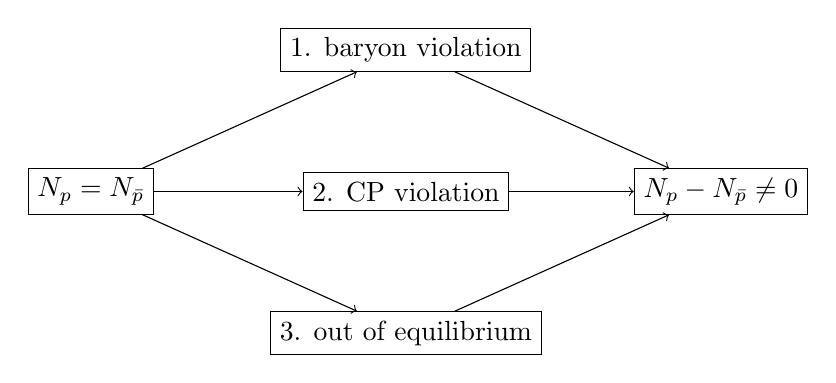
\begin{tikzpicture}[scale=1.0]
\node[draw,rectangle] (s) at (-4,0) {$N_p=N_{\bar p}$};
\node[draw,rectangle] (c1) at (0,1.8) {1. baryon violation};
\node[draw,rectangle] (c2) at (0,0) {2. CP violation};
\node[draw,rectangle] (c3) at (0,-1.8) {3. out of equilibrium};
\node[draw,rectangle] (f) at (4,0) {$N_p-N_{\bar p}\neq 0$};

\draw[->] (s) -- (c1);
\draw[->] (s) -- (c2);
\draw[->] (s) -- (c3);
\draw[->] (c1) -- (f);
\draw[->] (c2) -- (f);
\draw[->] (c3) -- (f);
\end{tikzpicture}
\caption{Minimal logical reconstruction of the board discussion. A symmetric starting point can tilt into a nonzero asymmetry only if the relevant laws violate baryon number, distinguish particles from antiparticles, and operate during a nonequilibrium epoch.}
\end{figure}

The lecture treats this combination as extraordinarily robust. If these conditions are present at sufficiently high energy, then a tiny leftover asymmetry is not mysterious. If they are absent, the asymmetry is extraordinarily hard to obtain.

\section{Clarifications at the Edge of What We Know}

The closing third of the lecture widens the ring of discussion. It does not abandon baryogenesis; it asks what part of the argument is theorem, what part is experiment, and what part is still conjecture.

First comes the distinction between CP, time reversal, and CPT. The relevant exact theorem is CPT, not plain charge conjugation. The lecture's point is subtle but important. Condition 3 is \emph{not} a violation of CPT. To be out of equilibrium simply means that the actual history of the universe was not a static equilibrium history. The universe was expanding, and sufficiently early it was expanding rapidly enough to matter on microscopic time scales. That gives a real arrow in the history without implying that the time-reversed history would fail to satisfy the underlying equations. So one must not confuse
\begin{equation}
\text{out of equilibrium}
\end{equation}
with any violation of the CPT theorem.

Second comes the empirical status of baryon-number violation. This is the question mark. We have never directly observed a reaction in nature in which
\begin{equation}
B=(N_p+N_n)-(N_{\bar p}+N_{\bar n})
\end{equation}
changes. That may only mean that the relevant reactions are important at very high temperature and fantastically improbable at low energy. But at present it remains unobserved.

That is why proton decay occupies so much of the late discussion. If baryon number is not exact, then the proton ought in principle to be unstable. Yet it is astonishingly stable. Ordinary particle processes occur on absurdly short time scales, but the proton must live at least as long as the age of the universe, and in fact much longer. The lecture quotes the experimental lower bound at the order-of-magnitude level as
\begin{equation}
\tau_p \gtrsim 10^{34}\ \text{years}.
\end{equation}
Huge underground detectors, typically giant volumes of water instrumented with photodetectors, have searched for precisely this sort of event. So far, nothing has been seen.

This empirical tension is one reason the story remains interesting. It is easy to write down extensions of the standard model that violate baryon number. The hard part is to do so without making the proton decay much too fast.

Third comes gravity. At the level of microscopic particle collisions, gravity is negligible and does not run the bookkeeping. But it enters the story in two deeper ways. One is obvious: without gravitational expansion of the universe there would be no cosmological departure from equilibrium. The second is the black-hole thought experiment emphasized in the lecture. If a star carrying a huge positive baryon number collapses to a black hole and later evaporates mostly into low-energy thermal radiation, it becomes very hard to believe that baryon number can remain an exact conservation law forever. That is not a laboratory observation of baryon violation, but it is powerful theoretical pressure against exact baryon conservation.

Electric charge is different. The lecture makes this contrast very sharply. A charged black hole cannot simply forget its charge, because electric flux lines continue to extend to infinity and keep track of it. That is why charge conservation is treated as exact here while baryon-number conservation is treated as provisional.

The lecture also briefly cleans up two side issues. The electroweak restoration scale, around \(100\)--\(250\,\mathrm{GeV}\), belongs to known physics and may matter in more complete models, but it is not the dramatic step in this story. Dark matter, in most standard discussions, is more or less a spectator here; it may carry its own history, but it does not alter the basic baryogenesis logic being isolated in this lecture.

There is also an important retrospective remark near the end. Older versions of the problem were often posed upside down: why are there so many photons compared with protons? But once the adiabatic picture is taken seriously, that formulation loses much of its force. The entropy of the universe, which in this context is essentially the number of photons up to an order-one factor, does not seem to have been manufactured in some gigantic late burst. The sharper question is the opposite one: why was the asymmetry between particles and antiparticles so tiny? Why was the excess only one part in a billion?

\paragraph{Neutron coda.} The lecture closes with a short discussion of neutrons, and it is worth keeping only the central point. Neutron beta decay,
\begin{equation}
n\to p+e^-+\bar\nu,
\end{equation}
does \emph{not} violate baryon number; the neutron carries the same baryon number as the proton. A free neutron decays because its mass is slightly larger than that of the final state, which we may summarize schematically as
\begin{equation}
m_n \gtrsim m_p+m_e+m_\nu.
\end{equation}
The available energy is small, and that small phase space contributes to the long lifetime of the free neutron. If the neutron is bound inside a nucleus, binding energy can remove the available decay energy:
\begin{equation}
M_{\mathrm{bound}} \approx m_n+m_p-\frac{E_{\mathrm{bind}}}{c^2}.
\end{equation}
That is why a bound neutron may be stable even though a free neutron is not. This is not part of baryogenesis proper, but it neatly separates an allowed weak decay from the genuinely hypothetical baryon-violating reactions that baryogenesis would require.

\section{Summary}

The lecture begins with visibility and ends with asymmetry. Looking outward takes us to earlier and hotter epochs; last scattering marks the transition from opaque ionized plasma to transparent neutral matter. Going still farther back, known atomic, nuclear, and particle physics lead us to a hot soup in which electrons and positrons, and later quarks and antiquarks, are produced in nearly equal numbers.

When we then run the movie forward, the essential mechanism is freeze-out. As thresholds are crossed, inverse production shuts off while annihilation continues, and matched particle--antiparticle pairs disappear into photons. The difference \(N_p-N_{\bar p}\) is not created by that process; it is preserved by it. The present photon excess,
\begin{equation}
\frac{N_\gamma}{N_p}\sim 10^9\text{--}10^{10},
\end{equation}
therefore tells us that the primordial asymmetry was only about one part in a billion.

That is why the lecture lands on baryogenesis. Ordinary cooling cannot generate the asymmetry within tested particle physics, and statistical fluctuations are far too small. To tilt a symmetric universe into a matter-dominated one, the laws must violate baryon number, distinguish particles from antiparticles, and act during a nonequilibrium epoch. Of these ingredients, the decisive missing empirical piece is still direct baryon-number violation. The structure of the story is compelling; the scale of the answer is plausible; but the most important experimental confirmation remains to be seen.
